\section{Zielsetzung}

In diesem Versuch wird die Beugungsfigur bei Beugung von Licht am Einzelspalt und
am Doppelspalt untersucht.

\section{Theorie}

Beugung von Licht passiert immer dann, wenn Licht durch eine Öffnung hindurchtritt,
der kleiner als der Strahlendurchmesser ist. Diese Beugung lässt sich erklären, wenn
Licht als eine Welle auffasst wird. Unter dieser Annahme lassen sich Beugungsphänomene
mit dem Huygenschen Prinzip erklären. Dieses Besagt, dass an jedem Punkt
einer Wellenfront eine neue Kugelwelle entsteht. Diese Elementarwellen überlagern
sich dann zu einer neuen Wellenfront.

In diesem Versuch wird die Fraunhofersche Lichtbeugung betrachtet. Bei diesem Versuchsaufbau
liegt die Lichtquelle im Unendlichen, dass sich ein Paralleles Lichtbündel ergibt und
die Beobachtungsebene liegt auch quasi im Unendlichen, oder ist in Realität weit von
dem Spalt entfernt. Eine Skizze dieser Versuchsanordnung ist in Abbildung \ref{abb:1}
abgebildet.

\begin{figure}[H]
  \centering
  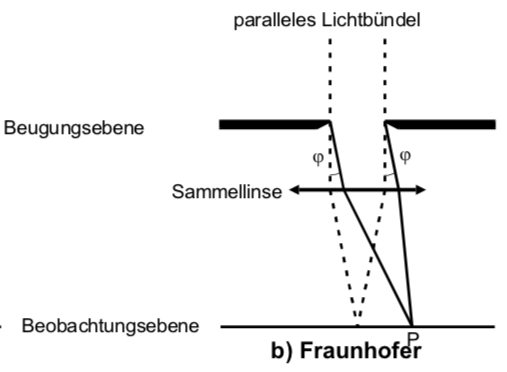
\includegraphics[width=10cm, height=7cm]{content/Frauenhofer.png}
  \caption{Frauenhofersche Beugung am Spalt \cite{1}.}
  \label{abb:1}
\end{figure}

Der Vorteil bei dieser Art von Beugung ist, dass alle Strahlen unter dem selben Winkel
$\varphi$ gebeugt werden. Wird nun das Huygensche Prinzip auf diese Beugung angewandt
folgt, dass wenn einzelne Strahlenbündel betrachtet werden, sie einen Wegunterschied $s$
haben zu einem beliebigen Punkt auf der Beobachtungsebene. Aufgrund dieses Wegunterschiedes $s$
haben diese Strahlenbündel eine Phasendifferenz

\begin{equation*}
  \delta = \frac{2 \pi s}{\lambda} = \frac{2 \pi x \sin(\varphi)}{\lambda}.
\end{equation*}

Dabei ist $\lambda$ die Wellenlänge des Lichtes und $x$ ist der Abstand der
betrachteten Strahlenbündel. Eine Skizze dieser Überlegung ist in
Abbildung \ref{abb:2} gezeigt.

\begin{figure}[H]
  \centering
  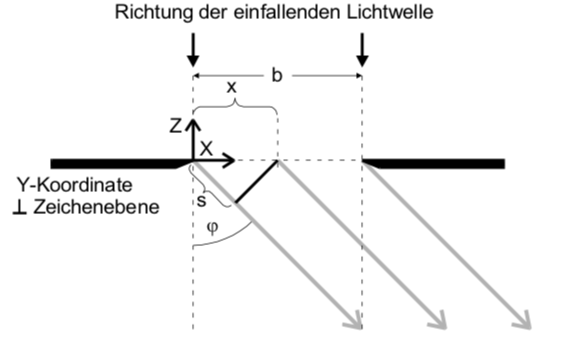
\includegraphics[width=10cm, height=7cm]{content/Phasendifferenz.png}
  \caption{Überlegung zur Herleitung der Phasenbeziehung bei Beugung am Spalt \cite{1}.}
  \label{abb:2}
\end{figure}

Nun fällt eine ebene Welle auf den Spalt ein mit der Feldstärke

\begin{equation*}
  A(z,t) = A_0 \exp\left(i\left(\omega t - \frac{2 \pi z}{\lambda} + \delta\right)\right).
\end{equation*}

Damit lässt sich eine Gleichung für die Amplitude $B$, nach der Beugung, in Abhängigkeit von $\varphi$ herleiten
durch Integrieren der Funktion $A(z,t)$ über die gesamte Spaltbreite. Es ergibt sich

\begin{equation*}
  B(z,t,\varphi) = A_0 \exp\left(i\left(\omega t - \frac{2 \pi z}{\lambda}\right)\right)
  \cdot \exp\left(\frac{\pi i b \sin(\varphi)}{\lambda}\right) \cdot \frac{\lambda}{\pi \sin(\varphi)}
  \sin\left(\frac{\pi b \sin(\varphi)}{\lambda}\right).
\end{equation*}

Da die komplexen Exponentialfunktionen keinen Einfluss auf die Amplitude haben, da es
lediglich Phasenfunktionen sind ergibt sich für die Amplitude

\begin{equation*}
  B(\varphi) = A_0 b \frac{\sin(\eta)}{\eta} \, \, \, \text{mit} \, \, \, \eta = \frac{\pi b \sin(\varphi)}{\lambda}.
\end{equation*}


Bei Lichtmessungen ist es nur möglich die Intensität zu messen. Mit dem Zusammenhang
$I(\varphi) \propto B(\varphi)^2$ ergibt sich für die Intensität

\begin{equation}
  I(\varphi) = A_0^2 b^2 \frac{\sin^2(\eta)}{\eta^2}.
  \label{eq:1}
\end{equation}

Die Beugung an einem Doppelspalt lässt sich auch als Überlagerung von Beugung an zwei
einzelnen Spalten betrachten. Damit folgt für die Intensität in diesem Fall

\begin{equation}
  I(\varphi) = 4 \cdot \cos^2\left(\frac{\pi s \sin(\varphi)}{\lambda}\right) \cdot
  \left(\frac{\lambda}{\pi b \sin(\varphi)}\right)^2 \cdot \sin^2\left(\frac{\pi b \sin(\varphi)}{\lambda}\right).
  \label{eq:2}
\end{equation}
